\documentclass{standalone}
\usepackage{tikz}
\usetikzlibrary{patterns, positioning}


\begin{document}
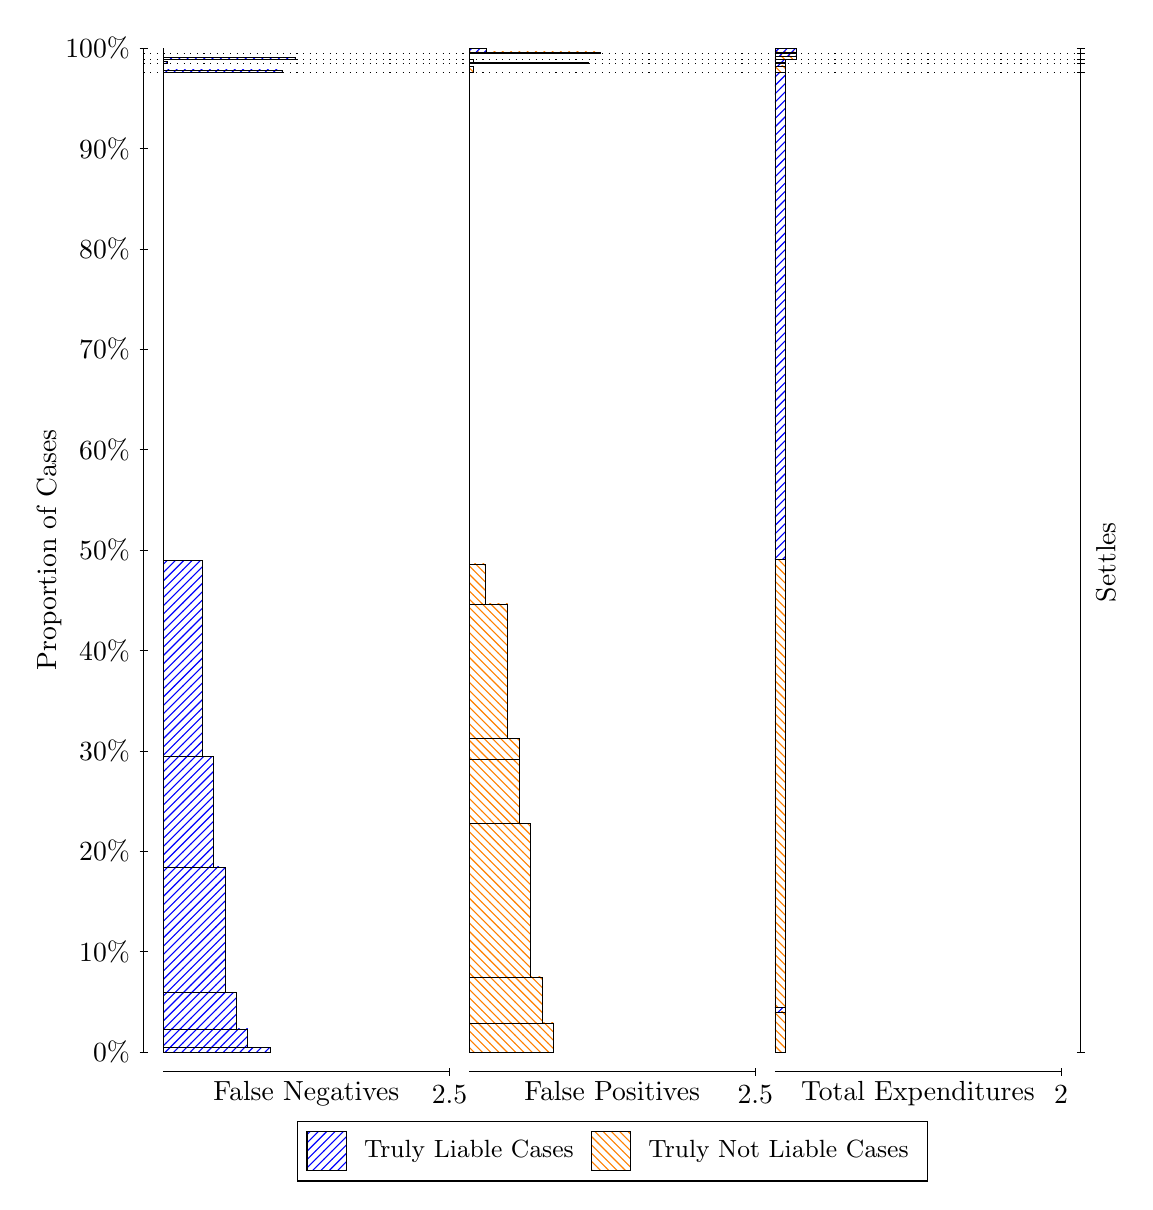
\begin{tikzpicture}
\draw[black, very thin] (1.5,1.75) -- (1.5,14.5);
\node[rotate=90, text=black, anchor=center] at (0.3, 8.125) {Proportion of Cases};
\draw[black, very thin] (1.45,1.75) -- (1.55,1.75);
\node[text=black, anchor=east] at (1.45, 1.75) {0\%};
\draw[black, very thin] (1.45,3.025) -- (1.55,3.025);
\node[text=black, anchor=east] at (1.45, 3.025) {10\%};
\draw[black, very thin] (1.45,4.3) -- (1.55,4.3);
\node[text=black, anchor=east] at (1.45, 4.3) {20\%};
\draw[black, very thin] (1.45,5.575) -- (1.55,5.575);
\node[text=black, anchor=east] at (1.45, 5.575) {30\%};
\draw[black, very thin] (1.45,6.85) -- (1.55,6.85);
\node[text=black, anchor=east] at (1.45, 6.85) {40\%};
\draw[black, very thin] (1.45,8.125) -- (1.55,8.125);
\node[text=black, anchor=east] at (1.45, 8.125) {50\%};
\draw[black, very thin] (1.45,9.4) -- (1.55,9.4);
\node[text=black, anchor=east] at (1.45, 9.4) {60\%};
\draw[black, very thin] (1.45,10.675) -- (1.55,10.675);
\node[text=black, anchor=east] at (1.45, 10.675) {70\%};
\draw[black, very thin] (1.45,11.95) -- (1.55,11.95);
\node[text=black, anchor=east] at (1.45, 11.95) {80\%};
\draw[black, very thin] (1.45,13.225) -- (1.55,13.225);
\node[text=black, anchor=east] at (1.45, 13.225) {90\%};
\draw[black, very thin] (1.45,14.5) -- (1.55,14.5);
\node[text=black, anchor=east] at (1.45, 14.5) {100\%};

\draw[black, very thin] (13.4,1.75) -- (13.4,14.5);
\draw[black, very thin] (13.35,1.75) -- (13.45,1.75);
\node[anchor=west] at (13.35, 1.75) {};
\draw[black, very thin] (13.35,14.192) -- (13.45,14.192);
\node[anchor=west] at (13.35, 14.192) {};
\draw[black, very thin] (13.35,14.304) -- (13.45,14.304);
\node[anchor=west] at (13.35, 14.304) {};
\draw[black, very thin] (13.35,14.352) -- (13.45,14.352);
\node[anchor=west] at (13.35, 14.352) {};
\draw[black, very thin] (13.35,14.427) -- (13.45,14.427);
\node[anchor=west] at (13.35, 14.427) {};
\draw[black, very thin] (13.35,14.5) -- (13.45,14.5);
\node[anchor=west] at (13.35, 14.5) {};

\draw[black, very thin, pattern color=blue, pattern=north east lines] (1.75,1.75) rectangle (3.1125,1.8106);
\draw[black, very thin, pattern color=blue, pattern=north east lines] (1.75,1.8106) rectangle (2.8218,2.0446);
\draw[black, very thin, pattern color=blue, pattern=north east lines] (1.75,2.0446) rectangle (2.6765,2.5073);
\draw[black, very thin, pattern color=blue, pattern=north east lines] (1.75,2.5073) rectangle (2.5312,4.1016);
\draw[black, very thin, pattern color=blue, pattern=north east lines] (1.75,4.1016) rectangle (2.3858,5.502);
\draw[black, very thin, pattern color=blue, pattern=north east lines] (1.75,5.502) rectangle (2.2405,7.9921);
\draw[black, very thin, pattern color=orange, pattern=north west lines] (1.75,7.9921) rectangle (1.75,14.192);
\draw[black, very thin, pattern color=blue, pattern=north east lines] (1.75,14.192) rectangle (3.2578,14.221);
\draw[black, very thin, pattern color=orange, pattern=north west lines] (1.75,14.221) rectangle (1.75,14.304);
\draw[black, very thin, pattern color=blue, pattern=north east lines] (1.75,14.304) rectangle (1.8045,14.334);
\draw[black, very thin, pattern color=orange, pattern=north west lines] (1.75,14.334) rectangle (1.75,14.352);
\draw[black, very thin, pattern color=blue, pattern=north east lines] (1.75,14.352) rectangle (3.4213,14.377);
\draw[black, very thin, pattern color=orange, pattern=north west lines] (1.75,14.377) rectangle (1.75,14.427);
\draw[black, very thin, pattern color=orange, pattern=north west lines] (1.75,14.427) rectangle (1.75,14.452);
\draw[black, very thin, pattern color=blue, pattern=north east lines] (1.75,14.452) rectangle (1.75,14.5);
\draw[black, very thin, pattern color=orange, pattern=north west lines] (5.6333,1.75) rectangle (6.7052,2.1188);
\draw[black, very thin, pattern color=orange, pattern=north west lines] (5.6333,2.1188) rectangle (6.5598,2.7031);
\draw[black, very thin, pattern color=orange, pattern=north west lines] (5.6333,2.7031) rectangle (6.4145,4.6527);
\draw[black, very thin, pattern color=orange, pattern=north west lines] (5.6333,4.6527) rectangle (6.2692,5.4654);
\draw[black, very thin, pattern color=orange, pattern=north west lines] (5.6333,5.4654) rectangle (6.2692,5.7364);
\draw[black, very thin, pattern color=orange, pattern=north west lines] (5.6333,5.7364) rectangle (6.1238,7.4395);
\draw[black, very thin, pattern color=orange, pattern=north west lines] (5.6333,7.4395) rectangle (5.8332,7.9498);
\draw[black, very thin, pattern color=blue, pattern=north east lines] (5.6333,7.9498) rectangle (5.6333,14.192);
\draw[black, very thin, pattern color=orange, pattern=north west lines] (5.6333,14.192) rectangle (5.6878,14.274);
\draw[black, very thin, pattern color=blue, pattern=north east lines] (5.6333,14.274) rectangle (5.6333,14.304);
\draw[black, very thin, pattern color=orange, pattern=north west lines] (5.6333,14.304) rectangle (7.1412,14.321);
\draw[black, very thin, pattern color=blue, pattern=north east lines] (5.6333,14.321) rectangle (5.6878,14.352);
\draw[black, very thin, pattern color=orange, pattern=north west lines] (5.6333,14.352) rectangle (5.6333,14.401);
\draw[black, very thin, pattern color=blue, pattern=north east lines] (5.6333,14.401) rectangle (5.6333,14.427);
\draw[black, very thin, pattern color=orange, pattern=north west lines] (5.6333,14.427) rectangle (7.3047,14.452);
\draw[black, very thin, pattern color=blue, pattern=north east lines] (5.6333,14.452) rectangle (5.8513,14.5);
\draw[black, very thin, pattern color=orange, pattern=north west lines] (9.5167,1.75) rectangle (9.6529,2.2603);
\draw[black, very thin, pattern color=blue, pattern=north east lines] (9.5167,2.2603) rectangle (9.6529,2.3209);
\draw[black, very thin, pattern color=orange, pattern=north west lines] (9.5167,2.3209) rectangle (9.6529,8.0105);
\draw[black, very thin, pattern color=blue, pattern=north east lines] (9.5167,8.0105) rectangle (9.6529,14.192);
\draw[black, very thin, pattern color=orange, pattern=north west lines] (9.5167,14.192) rectangle (9.6529,14.274);
\draw[black, very thin, pattern color=blue, pattern=north east lines] (9.5167,14.274) rectangle (9.6529,14.304);
\draw[black, very thin, pattern color=orange, pattern=north west lines] (9.5167,14.304) rectangle (9.6529,14.321);
\draw[black, very thin, pattern color=blue, pattern=north east lines] (9.5167,14.321) rectangle (9.6529,14.352);
\draw[black, very thin, pattern color=orange, pattern=north west lines] (9.5167,14.352) rectangle (9.7892,14.401);
\draw[black, very thin, pattern color=blue, pattern=north east lines] (9.5167,14.401) rectangle (9.7892,14.427);
\draw[black, very thin, pattern color=orange, pattern=north west lines] (9.5167,14.427) rectangle (9.7892,14.452);
\draw[black, very thin, pattern color=blue, pattern=north east lines] (9.5167,14.452) rectangle (9.7892,14.5);
\draw[black, dotted] (1.5,14.192) -- (13.4,14.192);
\draw[black, dotted] (1.5,14.304) -- (13.4,14.304);
\draw[black, dotted] (1.5,14.352) -- (13.4,14.352);
\draw[black, dotted] (1.5,14.427) -- (13.4,14.427);
\draw[black, very thin] (1.75,1.5) -- (5.3833,1.5);
\node[text=black, anchor=north] at (3.5667, 1.5) {False Negatives};
\draw[black, very thin] (5.3833,1.45) -- (5.3833,1.55);
\node[text=black, anchor=north] at (5.3833, 1.45) {2.5};

\draw[black, very thin] (5.6333,1.5) -- (9.2667,1.5);
\node[text=black, anchor=north] at (7.45, 1.5) {False Positives};
\draw[black, very thin] (9.2667,1.45) -- (9.2667,1.55);
\node[text=black, anchor=north] at (9.2667, 1.45) {2.5};

\draw[black, very thin] (9.5167,1.5) -- (13.15,1.5);
\node[text=black, anchor=north] at (11.333, 1.5) {Total Expenditures};
\draw[black, very thin] (13.15,1.45) -- (13.15,1.55);
\node[text=black, anchor=north] at (13.15, 1.45) {2};

\node[text=black, centered, rotate=90] at (13.72, 7.971) {Settles};





\draw (7.449999999999999,1.5) node[draw=none] (baseCoordinate) {};
\begin{scope}[align=center]
        \matrix[scale=0.5, draw=black, below=0.5cm of baseCoordinate, nodes={draw}, column sep=0.1cm]{
            \node[rectangle, draw, minimum width=0.5cm, minimum height=0.5cm, pattern color=blue, pattern=north east lines] {}; &
            \node[draw=none, font=\small, text=black] (B) {Truly Liable Cases}; &
            \node[rectangle, draw, minimum width=0.5cm, minimum height=0.5cm, pattern color=orange, pattern=north west lines] {}; &
            \node[draw=none, font=\small, text=black] (B) {Truly Not Liable Cases}; \\
            };
\end{scope}

\end{tikzpicture}
\end{document}